% file: 3-2-greedy/deadline-first-swap-long.tex

\documentclass[tikz]{standalone}

\usetikzlibrary{positioning, shapes.multipart}

\begin{document}
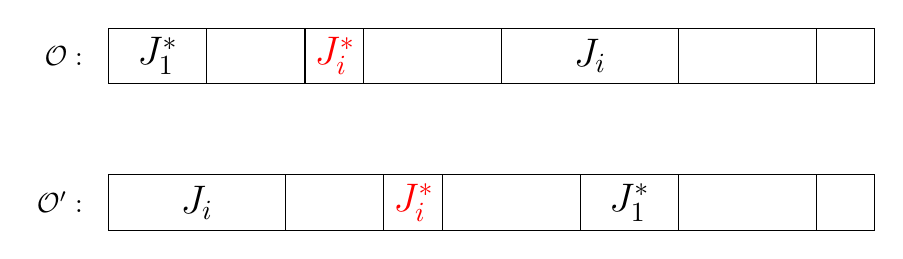
\begin{tikzpicture}[nodesplit/.style = {rectangle split, rectangle split parts = 7, draw, 
  	anchor = center, rectangle split horizontal, align = center, font = \Large}]
  \node (before) [nodesplit]
  {\nodepart[text width = 1.0cm]{one}$J_1^{\ast}$
   \nodepart[text width = 1.0cm]{two}
   \nodepart[text width = 0.5cm]{three}\textcolor{red}{$J_{i}^{\ast}$}
   \nodepart[text width = 1.50cm]{four}
   \nodepart[text width = 2.0cm]{five}$J_i$
   \nodepart[text width = 1.5cm]{six}
   \nodepart[text width = 0.5cm]{seven}
  };
   
  \node (o) [left = 0.20cm of before] {$\mathcal{O}:$};

  \node (after) [below = 1.5cm of before, nodesplit]
  {\nodepart[text width = 2.0cm]{one}$J_i$
   \nodepart[text width = 1.0cm]{two}
   \nodepart[text width = 0.5cm]{three}\textcolor{red}{$J_{i}^{\ast}$}
   \nodepart[text width = 1.50cm]{four}
   \nodepart[text width = 1.0cm]{five}$J_1^{\ast}$
   \nodepart[text width = 1.5cm]{six}
   \nodepart[text width = 0.5cm]{seven}
  };

  \node (o') [left = 0.20cm of after] {$\mathcal{O'}:$};
\end{tikzpicture}
\end{document}
